\chapter{OpenCAL OpenCL version}\label{ch:opencal-cl}

This chapter introduces OpenCAL-CL, a porting of OpenCAL in
OpenCL. OpenCL is an open standard for parallel programming defined by the
Khronos Group, that also defines other open standards like OpenGL and
Vulkan. Besides computational efficiency, one of the main advantages
of OpenCL is portability. In fact, OpenCL allows to run programs across
heterogeneous processors, like Central Processing Units (CPUs),
Graphics Processing Units (GPUs), Digital Signal Processors (DSPs),
and Field-Programmable Gate Arrays (FPGAs).

OpenCAL-CL inherits many OpenCAL features, by also adding parallel
computation capability thanks to the adoption of OpenCL. Statements
convention is similar to the one adopted in OpenCAL and OpenCAL-OMP,
with the peculiarity that the \verb'calcl' and \verb'CALCL' prefixes
are adopted for functions and data types, respectively, while the
\verb'CALCL_' prefix is used for constants. The active cells
optimization is fully supported, while a main difference with respect
to OpenCAL and OpenCAL-OMP is that OpenCAL-CL does not support unsafe
operations in the current version. Another main difference is that the
application is subdivided in two parts, one running on the CPU and one
running in parallel on a so called compliant device, like the ones
cited above. However, parallelism is almost transparent to the
user.

This Chapter introduces OpenCAL-CL by examples. After a brief
introduction to both OpenCL and OpenCAL-CL, in which both host and
device-side CA development is outlined, the implementation of the
$Life$ and $SciddicaT_{naive}$ 2D CA is presented. The implementation
of the $mod2$ 3D CA is also shown. The last two examples also deal
with OpenCAL-GL and show how to integrate a basic OpenGL/GLUT
visualization system in both 2D and 3D OpenCAL-CL applications.


\section{A brief introduction to OpenCL and OpenCAL-CL}\label{sec:opencalclstructure}

In order to better understand how OpenCAL-CL works, it is necessary to
introduce some OpenCL concepts. In OpenCL, data exchange and kernels
execution are managed thanks to an OpenCL \emph{context}. In
particular, the host application links kernels into one or more
containers, called \emph{programs}. The program therefore connects
kernels with the data to be processed and dispatches them to a special
OpenCL structure called \emph{command queue}. This is necessary
because only enqueued kernels are actually executed. Figure
\ref{fig:GeneralStructure} shows the general structure of an OpenCL
application. The context contains all the devices, command queues and
kernels; each device has its own command queue and each command queue
contains the kernels to be executed on the corresponding device.

\begin{figure}[tp]
  \begin{center}
    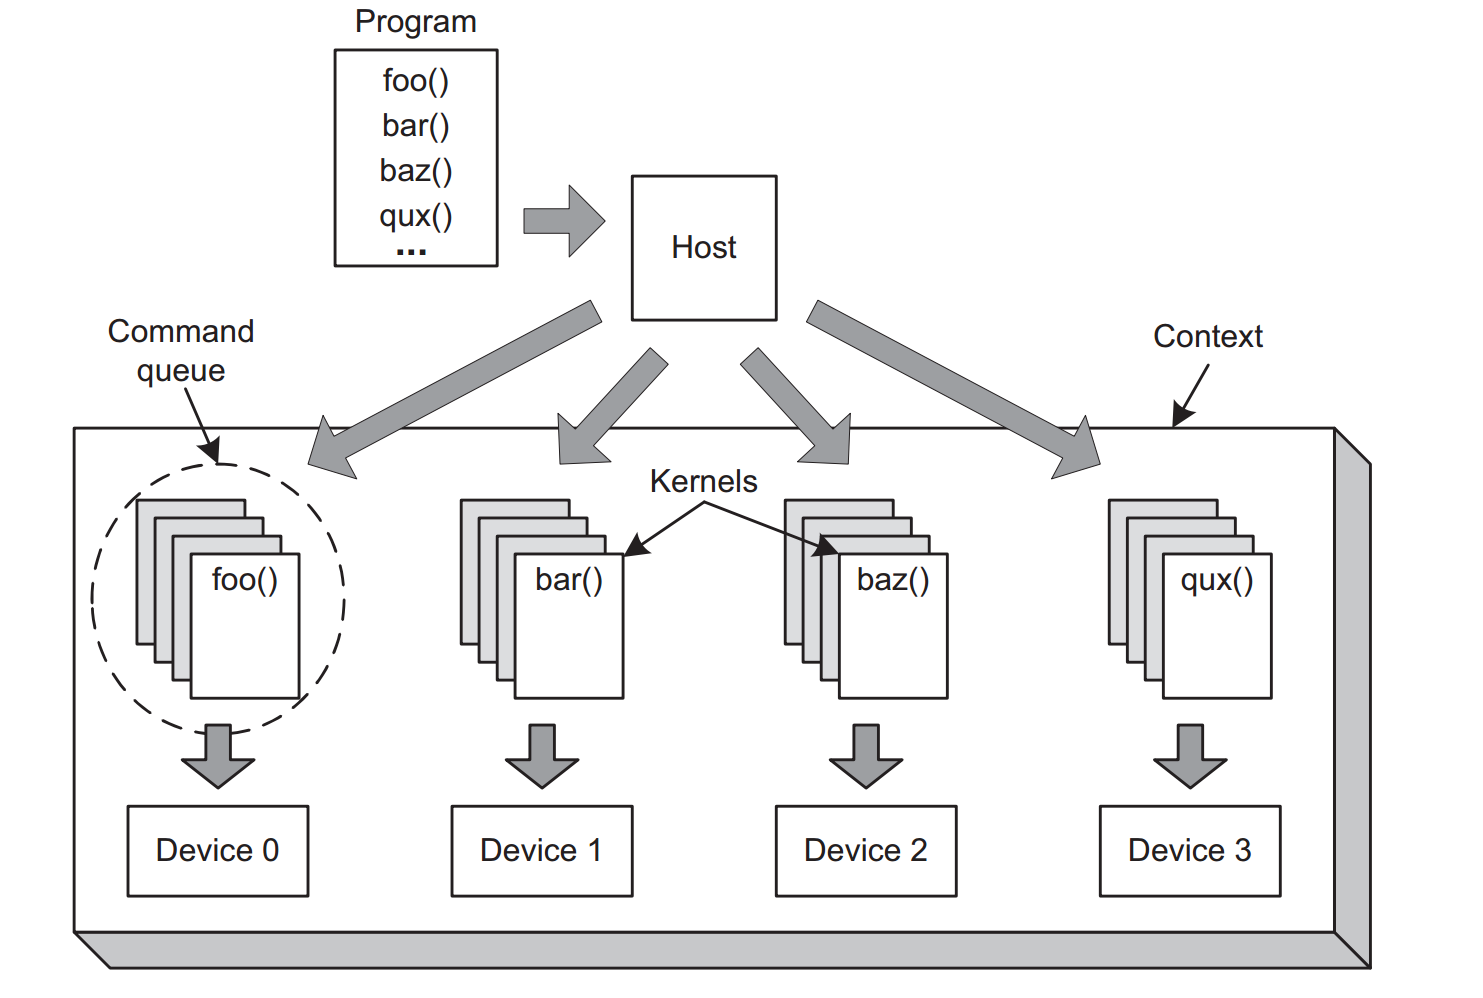
\includegraphics[width=12cm]{./images/OpenCAL-CL/kernelDistribution}
    \caption{General structure of a OpenCL program, from \emph{OpenCL
        in Action: How to accelerate graphics and computations},
      Matthew Scarpino, Manning Pubblication, ISBN-13:
      860-1400825129.}
    \label{fig:GeneralStructure}
  \end{center}
\end{figure}

As already stated, OpenCAL-CL, as well as OpenCL based applications,
are subdivided in two parts: the \emph{host application}, running on
the CPU, and the \emph{device application}, running on a compliant
computational device (e.g. a Nvidia or AMD GPU). Two CA objects are
therefore considered, one allocated host-side, while the other on the
compliant device. The host CA object is defined as in OpenCAL and
OpenCAL-OMP, while elementary processes, and possibly other global
functions like init, steering, and stop condition functions, are
registered to the device CA, to be executed in parallel. Accordingly,
they must be defined as OpenCL \emph{kernels}. As a consequence,
developers have to be able to write some minimal OpenCL code to
implement them. However, OpenCAL-CL hides lots of parallel aspects to
the user (e.g., the simulation loop is internally managed by the
library) and also simplifies data exchange between host and device.

As regards computational aspects, a number of threads equal to the
number of CA cells are executed in parallel for each computational
step. Each thread applies the CA elementary processes on a specific
cell, in the order they have been registered to the device-side CA. In
other words, OpenCAL-CL adopts the so called one thread-one cell
execution execution policy. According to OpenCL, threads are grouped
into workgroups. Threads within a workgroup can share information on a
local memory and also synchronize each other. Moreover, global data
can be shared thanks to the device global memory, which however is
slower than the local one. Eventually, threads can be globally
synchronized when kernels execution terminates and the control
returns to the host application.

In OpenCAL-CL many of the above aspects are completely transparent to
the user. In particular, the number of threads to be executed is set
by the library, as well as threads grouping into
workgroups. Eventually, even data exchange between host and device is
completely transparent to the user, with the exception that kernels have
to receive data which was not registered into the host-side CA model.

%% In the following sections, both device- and host-side OpenCAL-CL
%% programming are briefly introduced. The 2D version of OpenCAL-CL is
%% here considered for the proposed examples and discussions. However,
%% note that the same considerantion also holds for the 3D and also any
%% data type, constant and function presented for the 2D case have a 3D
%% equivalent version.


\subsection{OpenCAL-CL device-side Programming}

As already mentioned, functions that can be executed on an OpenCL
compliant device are called kernels. In order to explain how to write
an OpenCAL-CL based kernel, let's consider the example in Listing
\ref{lst:OpenCAL-CL-kernel}.

First of all, the \verb'calcl2D.h' header file must be included (line
1). Accordingly to OpenCL, each kernel definition must start with the
\verb'__kernel' keyword (line 8). However, differently to OpenCL,
where a kernel can have no parameters, each OpenCAL-CL kernel must
have at least the \verb'__CALCL_MODEL_2D' parameter. Actually, it is a
macro-like C object defining a list of pre-fixed typed parameters,
needed to let the kernel to know any data about the CA model, like
substates and the neighbourhood, beside others. Kernels can also take other
parameters, as in the example in Listing
\ref{lst:Another-OpenCAL-CL-kernel}. In the specific case, the
\verb'Pepsilon' parameter is allocated in the global memory of the
compliant device. It is also possible to allocate kernel parameters in
the faster local memory, which is shared by threads belonging to the
same work group, by means of the OpenCL \verb'__local'
keyword. Eventually, kernel parameters can also be private to the
current thread by means of the \verb'__private' keyword, as shown in
Listing \ref{lst:kernel-private-parameter}. The same holds for
variables defined inside the kernel body where the above cited
\verb'__global', \verb'__local' and \verb'_private' memory level
qualifiers can be used. Note that both kernel parameters and variables
declared without any memory level qualifier are implicitly considered
as private, as in the case of variables at lines 15 and 16 of Listing
\ref{lst:OpenCAL-CL-kernel}.

\begin{lstlisting}[float,floatplacement=H, label=lst:OpenCAL-CL-kernel, caption=Example of OpenCAL-CL kernel.]
  #include <OpenCAL-CL/calcl2D.h>

  // Define handles to CA substates
  //...
  #define Z 4
  #define H 5

  __kernel void calcl_kernel_example (__CALCL_MODEL_2D)
  {
    // Prevent the execution of more threads than the CA dimension
    calclThreadCheck2D();
    //...

    // Get the cell coordinates back
    CALint i = calclGlobalRow();
    CALint j = calclGlobalColumn();
    //...

    // Set a new value for the substate
    // whose handle is defined by H.
    // Please, note the usage of the
    // MODEL_2D macro-like object
    calclSet2Dr(MODEL_2D, H, i, j, h_next);
    //...
  }
\end{lstlisting}

The \verb'calclThreadCheck2D()' function at line 11 of Listing
\ref{lst:OpenCAL-CL-kernel} must be the first to be called into the
kernel, as it prevents the execution of a number of threads exceeding
the number of CA cells (Listing \ref{lst:OpenCAL-CL-kernel}, line
11). This is due to the fact that OpenCAL-CL can execute more threads
than the number of CA cells for better performance purposes. In the
case the active cells optimization is considered, the
\verb'calclActiveThreadCheck2D()' must be called instead of
\verb'calclThreadCheck2D()', to prevent the execution of a number of
threads exceeding the number of CA cells actually involved in
computation. The \verb'calclGlobalRow()' and
\verb'calclGlobalColumn()' functions (Listing
\ref{lst:OpenCAL-CL-kernel}, lines 15-16) are used to get the global
cell coordinates within the cellular space. The \verb'calclSet2Dr()'
function at line 23 updates the substate value for the central
cell. It is the kernel-side counterpart of the OpenCAL
\verb'calSet2Dr()' cell update functions. A complete list of functions
that can be used within OpenCAL-CL kernels are listed in Table
\ref{tab:kernel-utility-function}.


\begin{table}
  \centering
  \begin{footnotesize}
  \begin{tabular}{l|l}
    \hline
    Function & Brief description\\
    \hline
    \verb'calclGlobalRow()'               & Get the row coordinate for the current cell \\
    \verb'calclGlobalColumn()'            & Get the column coordinate for the current cell \\
    \verb'calclGlobalSlice()'             & Get the slice coordinate for the current cell \\
    \verb'calclLocalRow() '               & Get the local cell row coordinate within the OpenCL work group\\
    \verb'calclLocalColumn()'             & Get the local cell column coordinate within the OpenCL work group\\
    \verb'calclLocalSlice()'              & Get the local cell slice coordinate within the OpenCL work group\\
    \verb'calclGet[2D|3D][b|i|r]()'       & Get the substate value for the central cell\\
    \verb'calclGetX[2D|3D][b|i|r]()'      & Get the substate value for a neighboring cell\\
    \verb'calclGetRows()'                 & Get the number of CA rows \\
    \verb'calclGetColumns()'              & Get the number of CA columns \\
    \verb'calclGetSlices()'               & Get the number of CA slices \\
    \verb'calclgGetByteSubstatesNum()'    & Get the number of substates of \verb'CALbyte' type \\
    \verb'calclGetIntSubstatesNum()'      & Get the number of substates of \verb'CALint' type \\
    \verb'calclGetRealSubstatesNum()'     & Get the number of substates of \verb'CALreal' type \\
    \verb'calclGetCurrentByteSubstates()' & Get a pointer to the set of current layer of \verb'CALbyte' substates \\
    \verb'calclGetCurrentIntSubstates()'  & Get a pointer to the set of current layer of \verb'CALint' substates \\
    \verb'calclGetCurrentRealSubstates()' & Get a pointer to the set of current layer of \verb'CALreal' substates \\
    \verb'calclGetNextByteSubstates()'    & Get a pointer to the set of next layer of \verb'CALbyte' substates \\
    \verb'calclGetNextIntSubstates()'     & Get a pointer to the set of next layer of \verb'CALint' substates \\
    \verb'calclGetNnextRealSubstates()'   & Get a pointer to the set of next layer of \verb'CALreal' substates \\
    %% \verb'calclGetActiveCells()'          & Get a pointer to the set of active cells \\
    %% \verb'calclGetActiveCellsNum()'       & Get the number of active cells \\
    %% \verb'calclGetActiveCellsFlags()'     & Get a pointer to the set of active cells flags \\
    \verb'calclGetNeighborhood()'         & Get a pointer to the set of neighboring cells \\
    \verb'calclGetNeighborhoodID()'       & Get the neighbourhood ID (e.g. von Neumann, Moore, etc.) \\
    \verb'calclGetNeighborhoodSize()'     & Get the neighbourhood size \\
    \verb'calclGetBoundaryCondition()'    & Get the boundary condition (simple or cyclic) \\
    \verb'calclRunStop()'                 & Stops the simulation \\
    \verb'calclSet[2D|3D][b|i|r]()'       & Set the substate value for the central cell\\
    \verb'calclThreadCheck[2D|3D]()'      & Prevents unnecessary thread execution for 3D CA\\
    \verb'calclActiveThreadCheck[2D|3D]()'& Prevents unnecessary thread execution for 2D CA with active cells\\
    \hline
    \end{tabular}
    \end{footnotesize}
  \caption{Some OpenCAL-CL utility kernel functions.}
  \label{tab:kernel-utility-function}
\end{table}

Note that, functions that in OpenCAL were requiring a pointer to a CA
object, here take the \verb'MODEL_2D' macro-like C object in its
place, which implicitly defines a list of prefixed parameters needed
by the function (see e.g. line 23 of Listing
\ref{lst:OpenCAL-CL-kernel}). Moreover, substates are accessed by means
of numerical handles (cf. the second parameter of the
\verb'calclSet2Dr()' function at line 23), which have to be previously
defined in the kernel (cf. line 6). The criterion to be adopted
is very simple: handles are zero-based IDs. That is, zero (0) is used to link the
first host-side substate, i.e. the first substate added to the
host-side CA, one (1) is used to link the second substate added to the
host-side CA, and so on.

\begin{lstlisting}[float,floatplacement=H, label=lst:Another-OpenCAL-CL-kernel, caption={Another example of OpenCAL-CL kernel, with an additional global parameter.}]
  #include <calcl2D.h>
  //...

  __kernel void another_calcl_kernel_example (__CALCL_MODEL_2D, __global CALParameterr * Pepsilon)
  {

    //...
  }
\end{lstlisting}

\begin{lstlisting}[float,floatplacement=H, label=lst:kernel-private-parameter, caption={Another example of OpenCAL-CL kernel, with an additional private parameter.}]
  #include <calcl2D.h>
  //...

  __kernel void another_calcl_kernel_example (__CALCL_MODEL_2D, __private CALParameterr Pepsilon)
  {

    //...
  }
\end{lstlisting}



%% \subsection{Selection of the OpenCL compliant device}
\subsection{OpenCAL-CL host-side Programming}

An OpenCAL-CL host application is typically subdivided in the
following parts, which are described in the following sections:
\begin{itemize}
\item Definition of the host-side CA model;
\item Selection of the OpenCL compliant device;
\item Kernels reading and program generation;
\item Definition of the device-side CA model;
\item Kernels enqueuing;
\item Simulation execution on the previously selected compliant
  device.
\end{itemize}


\subsubsection{Definition of the host-side CA model}

The OpenCAL-CL host-side CA definition does not differ from what done
for the cases of OpenCAL (cf. Chapter \ref{ch:opencal}). Indeed, in
Listing \ref{lst:host-side-application}, a 2D host-side CA object is
declared by using the \verb'CALModel2D' OpenCAL data type (line 4),
and then initialized by means of the \verb'calCADef2D()' function
(line 11), exactly as in the serial version of OpenCAL. Note that the
\verb'calcl2D.h' OpenCAL-CL specific header file is included at line
1. This, in turn, includes the \verb'cal2D.h' header, so that it is
possible to use OpenCAL data types and functions from an OpenCAL-CL
host application.

\begin{lstlisting}[float,floatplacement=H, label=lst:host-side-application, caption={An example of OpenCAL-CL host-side application.}]
  #include <OpenCAL-CL/calcl2D.h>
  //...

  struct CALModel2D* hostCA;
  //...

  int main(int argc, char** argv)
  {
    //...

    hostCA = calCADef2D(ROWS, COLS, CAL_VON_NEUMANN_NEIGHBORHOOD_2D, CAL_SPACE_TOROIDAL, CAL_OPT_ACTIVE_CELLS);
    //...

  }
\end{lstlisting}


\subsubsection{Selection of the OpenCL compliant device}

OpenCAL-CL provides the \verb'CALOpenCL' structure that, together with
other utility functions, considerably simplifies platform, device, and
context management with respect to the native OpenCL API. Listing
\ref{lst:CALOpenCL} shows how to select a compliant device in
OpenCAL-CL.

\begin{lstlisting}[float,floatplacement=H, label=lst:CALOpenCL, caption=Access to platform and devices.]
  #include <OpenCAL-CL/calcl2D.h>
  //...

  int main (int argc, char** argv)
  {
    // Initilize a pointer to the CALCLManager structure
    CALCLManager * calcl_manager = calclCreateManager ();

    // get all available platforms
    calclInitializePlatforms ( calcl_manager );

    // Initialize the devices
    calclInitializeDevices ( calcl_manager );

    // Uncomment if platforms and devices are unknown
    //calclGetPlatformAndDeviceFromStdIn();

    // get the first device on the first platform
    // this call is unnecessary if calclGetPlatformsAndDeviceFromStandardInput() is used
    CALCLdevice device = calclGetDevice ( calcl_manager , 0, 0 );

    // create a context
    CALCLcontext context = calclCreateContext ( &device );

    // ...
  }
\end{lstlisting}

Line 7 declares a pointer to the \verb'CALCLManager' OpenCAL-CL data
type, and initializes it through the \verb'calclCreateManager()'
function. This object, \verb'calcl_manager', is then used as parameter
for the \verb'calclInitializePlatforms()' function (line 10), which
fills the object with the platforms available on the machine. Line 13
calls the \verb'calclInitializeDevices()' function, that initializes
the available devices, while line 20 selects one of them for kernel
execution. Specifically, an object of type \verb'CALCLdevice' is
declared and initialized by the function \verb'calclGetDevice()'. This
latter takes a pointer to a \verb'CALManager' object as first
parameter, while the second and third parameters specify the platform
and device to be selected, respectively. Since both platforms and
devices are identified by a 0-based index\footnote{In OpenCAL-CL
  platforms and devices are stored in a matrix where rows represent
  platforms and columns devices. Thus, to choose which platform and
  device to use for the computation, it is necessary to specify their
  indexes within the matrix. For example, at lines 15, we chose the
  platform number 0 and the device number 0. If we have a system with
  3 NVIDIA GPUs and 3 AMD GPUs, the library will have a $2 \times 3$
  size matrix, where 2 are the vendors (i.e., the platforms NVIDIA and
  AMD) and 3 are the GPUs for each platforms. If we want to run the
  program using the third AMD GPU, we can specify 1 and 2 as
  indices.}, statement at line 20 selects the first device belonging
to the first platform (e.g. a GTX 980 belonging to the NVIDIA CUDA
platform). If system platforms and devices are unknown, the
\verb'calclGetPlatformAndDeviceFromStdIn()' function can be used
alternatively to \verb'calclGetDevice()'. It prints all the available
platforms and devices to standard output and permits for their
interactive selection from standard input. Eventually, line 23 creates
an OpenCL context, based on the device previously selected. For this
purpose, an object of \verb'CALCLcontext' type is declared and defined
by means of the \verb'calclCreateContext()' function.

\subsubsection{Kernels reading and program generation}

After the compliant device has been selected and elementary processes
(and possibly other functions) implemented as kernels, these latter
can automatically be read and compiled through the
\verb'calclLoadProgram2D()' and \verb'calclLoadProgram3D()' functions
(cf. Listing \ref{lst:calclLoadProgram}). They take both the context
and device, and also the paths to directories containing the user
defined kernels and related headers (if any) as parameters, and
returns an OpenCL program\footnote{\texttt{CALCLprogram} redefines the
  \texttt{cl\_program} OpenCL type.}. All the files in the kernel
source directory are automatically considered, independently from
their name. Note that, since kernel headers are optional, the last
parameter can be \verb'NULL'.

\begin{lstlisting}[float,floatplacement=H, label=lst:calclLoadProgram, caption={The calclLoadProgram function. It loads and compiles kernels by returning an OpenCL program.}, numbers=none]
  CALCLprogram calclLoadProgram[2D|3D] (
    CALCLcontext context ,
    CALCLdevice device ,
    char * kernel_source_directory ,
    char * kernel_include_directory
  )
\end{lstlisting}

\subsubsection{Definition of the device-side CA model}

OpenCAL-CL allows for having a counterpart of the host-side CA to
device-side. Such a device-side CA is declared as a
\verb'CALCLModel2D' object and, beside managing all the CA components
device-side, also provides simulation execution features. Note
that, this is a main difference with respect to OpenCAL serial
version, where the simulation execution is managed by a
\verb'CALRun2D' complementary object.

To initialize the device-side CA object, the \verb'calclCADef2D'
function can be used (cf. Listing \ref{lst:calclCADef2D}; cf. also
Listing \ref{lst:calclCADef3D} for its 3D version). The first
parameter is a pointer to a \verb'CALModel2D', defined host side as in
the case of the serial implementation of OpenCAL (cf. Chapter
\ref{ch:opencal}). The second one is an OpenCL context, as well as the
third and fourth parameters are an OpenCL program and compliant
device, respectively.

%% The device-side CA object permits to equeue the defined kernels

\begin{lstlisting}[float,floatplacement=H, label=lst:calclCADef2D, caption=The calclCADef2D function., numbers=none]
  CALCLModel2D * calclCADef2D(
                   struct CALModel2D * host-model,
                   CALCLcontext context,
                   CALCLprogram program,
                   CALCLdevice device
  )
\end{lstlisting}

\begin{lstlisting}[float,floatplacement=H, label=lst:calclCADef3D, caption=The calclCADef3D function., numbers=none]
  CALCLModel3D * calclCADef3D(
                   struct CALModel3D * host-model,
                   CALCLcontext context,
                   CALCLprogram program,
                   CALCLdevice device
  )
\end{lstlisting}


\subsubsection{Kernels enqueuing}

Once compiled and grouped in a program, kernels can be
extracted in order to be attached to a command queue for
execution. The \verb'calclGetKernelFromProgram()' function can be used
to extract a kernel from an OpenCL program. It takes a pointer to the
program and the kernel name (cf. Listing
\ref{lst:calclGetKernelFromProgram}).

\begin{lstlisting}[float,floatplacement=H, label=lst:calclGetKernelFromProgram, caption={The calclGetKernelFromProgram kernel extraction function}., numbers=none]
  CALCLkernel calclGetKernelFromProgram (
    CALCLprogram * program,
    char * kernelName
  )
\end{lstlisting}

The function \verb'calclAddElementaryProcess2D' adds a new kernel to
the execution queue (cf. Listing
\ref{lst:calclAddElementaryProcess2D}; cf. also Listing
\ref{lst:calclAddElementaryProcess3D} for the 3D version), in a
transparent manner to the user. The function takes both a pointer to
host and device CA as parameter and also a pointer to an OpenCL
kernel.

\begin{lstlisting}[float,floatplacement=TH, label=lst:calclAddElementaryProcess2D, caption=The calclAddElementaryProcess2D() function., numbers=none]
  void calclAddElementaryProcess2D(
               CALCLModel2D * deviceCA,
               struct CALModel2D * hostCA,
               CALCLkernel * kernel
  );
\end{lstlisting}

\begin{lstlisting}[float,floatplacement=TH, label=lst:calclAddElementaryProcess3D, caption=The calclAddElementaryProcess3D() function., numbers=none]
  void calclAddElementaryProcess3D(
               CALCLModel3D * deviceCA,
               struct CALModel3D * hostCA,
               CALCLkernel * kernel
  );
\end{lstlisting}

Note that, if the kernel to be added has one or more parameters
(beside the mandatory \verb'__CALCL_MODEL_2D' one), they must be
passed to the device-side application. Passing a parameter to a
kernel is a operation which depends on how the parameter is declared, i.e., 
whether if as a pointer or not.

Let as consider the example in Listing
\ref{lst:Another-OpenCAL-CL-kernel}, where a parameter is declared as
a pointer to be stored into the device global memory. A double step
procedure must be used in this case. First, the
\verb'calclCreateBuffer()' function must be called. It takes the
OpenCL context, the address of the host parameter to be passed to the
kernel, and the dimension of the host parameter type, and returns an
object of type \verb'CALCLmem', which is a buffer containing the value
of the host-side parameter. This buffer is therefore used by the
\verb'calclSetKernelArg[2D|3D]()' functions, which actually perform
the data transmission to the device. They take the kernel to which send
the parameter, the parameter position within the kernel parameter list
(0 for the first one after the mandatory \verb'__CALCL_MODEL_2D'
parameter, 1 for the second, and so on), the \verb'CALCLmem'
dimension, and the address of the buffer containing the value for the
kernel parameter (cf. Listing \ref{lst:calclSetKernelArg2D}). Listing \ref{lst:calclKernelParameters} shows an example of how
parameters can be passed to a kernel with the above described method.

At the contrary, if the kernel parameter is not declared as a pointer,
like in the example in Listing \ref{lst:kernel-private-parameter}, the
above double step process is no longer necessary, since it is
sufficient to call the \verb'calclSetKernelArg[2D|3D]()' by specifying
the dimension of the actual type of the variable to be passed to the
kernel as third parameter .

%% calclSetKernelArg2D(&kernel_elem_proc_flow_computation, 1, sizeof(CALParameterr), &P.r);

\begin{lstlisting}[float,floatplacement=H, label=lst:calclSetKernelArg2D, caption=The calclSetKernelArg2D() function., numbers=none]
  int calclSetKernelArg[2D|3D](CALCLkernel* kernel,
                               cl_uint arg_index,
                               size_t arg_size,
                               const void *arg_value
  )
\end{lstlisting}


\begin{lstlisting}[float,floatplacement=H, label=lst:calclKernelParameters, caption=Passing parametrs to kernel.]
  #include <OpenCAL-CL/calcl2D.h>
  //...

  struct sciddicaTParameters {
    CALParameterr epsilon;
    //...
  } P;

  //...

  int main(int argc, char** argv)
  {
    //...
    CALCLmem bufferEpsilonParameter;
    //...

    bufferEpsilonParameter = calclCreateBuffer(context, &P.epsilon, sizeof(CALParameterr));
    calclSetKernelArg2D(&kernel_elem_proc_flow_computation, 0, sizeof(CALCLmem), &bufferEpsilonParameter);
    //...
  }
\end{lstlisting}



\begin{table}
  \centering
  \begin{footnotesize}
  \begin{tabular}{l|l}
    \hline
    Function & Brief description\\
    \hline
    \verb'calclAddInitFunc[2D|3D]'             & register a global kernel to be executed before simulation loop \\
    \verb'calclAddElementaryProcess[2D|3D]()'  & register an elementary process \\
    \verb'calclAddSteeringFunc[2D|3D]'         & register a global kernel to be executed after each step \\
    \verb'calclAddStopConditionFunc[2D|3D]()'  & register a global stop condition kernel callback \\
    \hline
    \end{tabular}
    \end{footnotesize}
  \caption{OpenCAL-CL host-side functions used to register elementary processes and global functions to the device-side CA.}
  \label{tab:XXX}
\end{table}


\begin{lstlisting}[float,floatplacement=H, label=lst:calclRun2D, caption=The calclRun2D() function., numbers=none]
  void calclRun2D(CALCLModel2D* deviceCA,
                  struct CALModel2D * hostCA,
                  unsigned int initialStep,
                  unsigned maxStep
  );
\end{lstlisting}

\begin{lstlisting}[float,floatplacement=H, label=lst:calclRun3D, caption=The calclRun3D() function., numbers=none]
  void calclRun3D(CALCLModel3D* deviceCA,
                  struct CALModel3D * hostCA,
                  unsigned int initialStep,
                  unsigned maxStep
  );
\end{lstlisting}


\subsubsection{Simulation execution on the compliant device}

The \verb'calclRun2D()' function (cf. Listing \ref{lst:calclRun2D};
cf. also Listing \ref{lst:calclRun2D} for the 3D version) runs the CA
simulation by executing all the defined kernels on the selected
compliant device. The first two parameters are pointers to a device
and host CA, respectively, while the last two are the initial and
final step for the simulation execution. If the last parameter is set
to \verb'CAL_RUN_LOOP', simulation never ends. In this case, to stop
the simulation, the user must define a stop condition criterion
through the \verb'calclAddStopConditionFunc2D()' function
(cf. \ref{lst:calclAddStopConditionFunc2D}, cf. also Listing
\ref{lst:calclAddStopConditionFunc3D} for the 3D version). Note that,
since the stop condition must be evaluated host side, it must be
implemented as a kernel. For this reason, the third parameter is a
pointer to an OpenCL kernel. Other kernels can be registered to the
device-side CA. Table \ref{tab:XXX} list the OpenCAL-CL that can be
used to register kernels to the device-side CA.


\begin{lstlisting}[float,floatplacement=H, label=lst:calclAddStopConditionFunc2D, caption=The calclAddStopConditionFunc2D function., numbers=none]
  void calclAddStopConditionFunc2D(
                 CALCLModel2D * deviceCA,
                 struct CALModel2D * hostCA,
                 CALCLkernel * kernel
  );
\end{lstlisting}

\begin{lstlisting}[float,floatplacement=H, label=lst:calclAddStopConditionFunc3D, caption=The calclAddStopConditionFunc3D function., numbers=none]
  void calclAddStopConditionFunc3D(
                 CALCLModel3D * deviceCA,
                 struct CALModel3D * hostCA,
                 CALCLkernel * kernel
  );
\end{lstlisting}


\section{Conway's Game of Life with OpenCAL-CL}\label{sec:calcl_life}

As already done in previous Chapters about OpenCAL and OpenCAL-OMP,
here we introduce OpenCAL-CL programming by implementing Conway's Game
of Life. The application is subdivided in two parts, one for the host
and one for the compliant device.

The host-side application, running on the CPU and controlling the
computation on the compliant device (e.g. a GPU), is shown in Listing
\ref{lst:calcl_life}.


\lstinputlisting[label=lst:calcl_life, caption=An OpenCAL-CL
  host-side implementation of the Conway's Game of
  Life.]{../opencal-examples/OpenCAL-CL/calcl_life/source/life.c}

Differently from the serial implementation, discussed in Section
\ref{sec:cal_life}, the OpenCAL-CL \verb'calcl2D.h' header file is
include at line 3. It, in turn, includes the \verb'cal2D.h' header,
needed to define the host-side CA model. The OpenCAL \verb'cal2DIO.h'
header is also included at line 4 for I/O operations.

At line 7, the path containing the kernels to be executed in parallel
on the compliant device is defined, while the name of the single
kernel considered in this example is defined at line 8. Lines 9-10
define the IDs of the OpenCL platform and device to be considered. For the sake of simplicity, in
this example the first device belonging to the first platform is
considered.

Lines 15-18 are needed to select the compliant device and to create an
OpenCL context. These statements widely simplify the device management
and can be considered as a kind of template to be used in each
OpenCAL-CL application. Indeed, they will also be adopted in the
subsequent examples.

Line 21 reads kernels (actually, just one in this example) from file
(contained in the directory specified at line 7), compile and groups
them into an OpenCL program, to be used later to extract kernels for
execution.

Lines 24-38 are equivalent to the serial implementation of $Life$. The
\verb'host_CA' host-side object is defined at line 24 and the \verb'Q'
substate declared at line 25. This latter is therefore registered to
the host-side CA at line 28. Eventually, a glider is defined at lines
34-38.

Line 41 defines the \verb'device_CA' device-side object. The
\verb'calclCADef2D()' function initializes the device-side CA, by
performing data transfer from host to device, in a transparent way to
the user. Note that this function implicitly registers each host-side
defined substate to the device object. However, to access the substate
device-side, the user have to define a numeric handle, as discussed
below.

In order to register an elementary process to the device-side CA,
where computation will take place, a preliminary operation must be
performed: the elementary process, which actually is an OpenCL kernel,
must be extracted from the previously compiled program. This operation
is done at line 44 by means of the
\verb'calclGetKernelFromProgram()'. It returns an OpenCL kernel which
is subsequently registered to the device CA by means of the
\verb'calclAddElementaryProcess2D()' function at line 47.

Lines 50 an 56 are used to save the CA state (represented by the
single \verb'Q' substate) before and after simulation execution,
respectively.

The CA simulation is executed by means of the \verb'calclRun2D()'
function at line 5. In this example, the only defined elementary
process is executed in parallel on the compliant device, in a
transparently way to the user.

Eventually, lines 59-61 perform memory deallocation for the previously
defined objects.

\lstinputlisting[label=lst:calcl_life_kernel, caption=The OpenCAL-CL kernel
  implementing the Conway's Game of Life elementary
  process.]{../opencal-examples/OpenCAL-CL/calcl_life/kernel/source/life.cl}

Listing \ref{lst:calcl_life_kernel} shows the OpenCAL-CL kernel
implementing the Conway's Game of Life transition function.

The \verb'calcl2D.h' is included at line 3, while the numeric \verb'Q'
handle is defined at line 5 to access the the \verb'Q' substate,
registered to the host CA and, implicitly, to the device CA at line 50
of Listing \ref{lst:calcl_life}. In this case, the handle takes the
value 0, being \verb'Q' the only considered substate. If more
substates would be considered, other numeric handles would be defined,
taking increasing values.

The elementary process is implemented within the
\verb'lifeTransitionFunction()' kernel, defined at lines 7-25. As
previously evidenced, it takes the \verb'__CALCL_MODEL_2D' macro,
which implicitly defines a set of parameters for the kernel.

Line 9 assures the execution of a number of concurrent threads equal to
the number of cells in the CA cellular space, while lines 11-12 get the
indexes corresponding to the integer coordinates of the cell the
kernel is going to process. In this way, the one thread-one cell
policy is simply obtained.

Line 14 gets the neighborhood size, while line 16 declares some
variables to be used later.

Lines 18-24 implement the $life$ transition rules. Note that, the
\verb'calclGetX2Di()' and \verb'calclSet2Di()' functions are here used
to access the substate values for the neighbouring cells and to set
the new state for the central cell. They correspond to the
\verb'calGetX2Di()' and \verb'calSet2Di()' OpenCAL functions, with the
difference that, in spite of taking a CA model as parameter, they take
the \verb'MODEL_2D' OpenCAL-CL macro.

Figures \ref{fig:life_0000} and \ref{fig:life_LAST} in Chapter
\ref{ch:opencal} show the initial and final configuration of Game of
Life as implemented in Listing \ref{lst:calcl_life}, respectively.


\section{SciddicaT}\label{sec:calcl_sciddicaT}
In the previous section we illustrated an OpenCAL-CL implementation of
a simple cellular automaton, namely the Conway’s Game of Life. Here,
we will deal with a more complex example, concerning the the
$SciddicaT_{naive}$ Cellular Automata model for landslide simulation,
already presented in Section \ref{sec:sciddicaT} together with its
serial implementation. Eventually, we will show how to combine the
OpenCAL-CL and OpenCAL-GL libraries to integrate an OpenGL/GLUT
visualization system.

\lstinputlisting[label=lst:calcl_gl_sciddicaT, caption=An OpenCAL-CL
  host-side implementation of the SciddicaT Cellular Automata model
  for landslide
  simulation.]{../opencal-examples/OpenCAL-CL/calcl_gl_sciddicaT/source/sciddicaT.c}

The host-side implementation of $SciddicaT_{naive}$ is shown in
Listing \ref{lst:calcl_gl_sciddicaT}. Lines 4-9 include some
headers. In particular, the \verb'cal2DIO.h' OpenCAL header is
included for I/O purposes, while the \verb'calcl2D.h' and
\verb'calgl2DRunCL.h' headers provide CA definition and graphic
rendering support for the OpenCAL-CL library. Eventually, the
\verb'calgl2D.h' and \verb'calgl2DWindow.h' OpenCAL-GL headers are
included, to complete the application support for 2D and 3D rendering.

Lines 12-21 provide definitions and are almost the same of the
serial implementation shown in Listing \ref{lst:cal_sciddicaT}. In
addition, \verb'GRAPHIC_UPDATE_INTERVAL' defines the interval (in
terms of computational steps) to be used for both data retrieval from
the OpenCL compliant device and visualization purposes.

Lines 24-34 provide other definitions, specifying kernels paths and
names. Note that, different paths are here defined, depending whether
the active cells optimization is considered or not
(cf. \verb'ACTIVE_CELLS', line 24). In the first case, an additional
kernel is defined at line 33.

Lines 37-47 define two data types for grouping CA substates and
parameters, while lines 50-54 declare host- and device-side CA
objects, substates, and parameters, besides the
\verb'calcl_device_manager' object, needed to select the OpenCL
compliant device.

In the main function, after OpenCL device, context and program
declarations, kernel variables are declared at lines 117-120, while
lines 121-122 declare buffers to be used for kernel parameter
settings.  The device manager is then defined at line 125, a device
selected by means of the \verb'calclGetPlatformAndDeviceFromStdIn()'
function at line 126. This latter prints all the available platforms
and devices to standard output and allows for their interactive
selection.

OpenCL kernels, implementing transition function elementary
processes and, optionally, other functions like global init or
steering, are read from files, compiled and grouped together into an
OpenCL container called program at line 130, with a single call to
\verb'calclLoadProgram2D()'.

The host-side CA is therefore defined at lines 133-137, and
substates registered at lines 140-145. Note that, the order in which
substates are registered, implicitly define the values to be assigned
to substate handles to refer related data device-side.

The initial configuration is defined at lines 148-152. The
\verb'calLoadSubstate2Dr()' function is here used to initialize two
substates from file, while the others are initialized through the
\verb'sciddicaTSimulationInit()' function at line 151. Note that, in
order to apply the initialization performed before to the substates
\emph{next working planes}, it is necessary to call
\verb'calUpdate2D()'\footnote{Note that, in the serial implementation
  of SciddicaT, this operation was performed automatically by the
  simulation object.}.

The device-side CA is defined at line 155. As for the case of Conway's
Game of Life, the \verb'calclCADef2D()' function initializes the
object, by performing data transfer from the host to the device memory,
in a transparent way to the user.

In order to be able to execute a simulation, transition function
elementary processes and global functions must be registered to the
device-side CA object. This is a two-step process: at first, kernels
are extracted from the OpenCL program by means of the
\verb'calclGetKernelFromProgram()' function (cf. e.g. line 158) and
therefore they are registered to the device-side CA object through the
\verb'calclAddElementaryProcess2D()' function (cf. e.g. line 172). In
the specific case of $SciddicaT_{naive}$, some elementary processes require
parameters, that are defined and set at lines 166-177 through the
\verb'calclCreateBuffer()' and \verb'calclSetKernelArg2D()' functions,
respectively (as described in Section
\ref{sec:opencalclstructure}). Eventually, the steering kernel is
registered at line 179 through the \verb'calclAddSteeringFunc2D()'
function.

Starting from line 182, an integration with the OpenCAL-GL library is
implemented in order to provide a minimal GLUT Graphical User
Interface and a simplified OpenGL 2D/3D visualization system to the
application. Firstly, an exit function is registered to the
application for memory release purposes at line 182 through the
\verb'atexit()' C function\footnote{This is necessary because, once
  entered the GLUT main loop, the GL Utility Toolkit does not return
  the control to the main application.}. The viewer is initialized at
line 186 by means of the \verb'calglInitViewer()' function, while the
next call is used to define a vertical layout for the two 2D and 3D
rendering objects, defined later at lines 190-191.

The rendering tree-based structures for the 3D and 2D rendering
objects are defined at lines 198-210 and 213-215, respectively. A
simulation object is then defined at line 194 by means of the
\verb'CALGLRun2D()' function and run on the OpenCL compliant device at
line 218 by means of the \verb'calglMainLoop2D()' function. This
latter executes kernels in parallel on the device by considering the
one thread-one cell policy, manages data retrieval from compliant
device to host at prefixed intervals (in terms of computational steps
- cf. the \verb'GRAPHIC_UPDATE_INTERVAL' definition at line 21), and
performs the graphic rending.

For further details about OpenCAL-GL, please refer Section \ref{sec:calgl_sciddicaT}.

\lstinputlisting[label=lst:calcl_gl_sciddicaT_kernels_header, caption={The SciddicaT
  kernels' header file, as implemented in
  OpenCAL-CL.}]{../opencal-examples/OpenCAL-CL/calcl_gl_sciddicaT/kernelActive/include/kernel.h}

\lstinputlisting[label=lst:calcl_gl_sciddicaT_kernels, caption=The OpenCAL-CL
  kernels implementing the SciddicaT elementary processes and
  steering.]{../opencal-examples/OpenCAL-CL/calcl_gl_sciddicaT/kernelActive/source/kernel_user.cl}

The device-side implementation of SciddicaT which take into account
the active cells optimization is shown in Listings
\ref{lst:calcl_gl_sciddicaT_kernels_header} and
\ref{lst:calcl_gl_sciddicaT_kernels} for kernels sources and header,
respectively. Non-optimized versions are here omitted for the sake of
shortness.

Line 3 includes the \verb'calcl2D.h' header, while line 6 define the
number of outflows considered in SciddicaT. Eventually, lines 7-12
define the substates handles. Here, handles are assigned by taking
into account the order in which they have been registered to the
host-side CA (cf. Listing \ref{lst:calcl_gl_sciddicaT}, lines
140-145).

As regards the kernels shown in Listings
\ref{lst:calcl_gl_sciddicaT_kernels}, they do not differ from that of
the Game of Life (cf. \ref{lst:calcl_life}). In fact, each kernel is
identified by the \verb'__kernel' keyword and, with the exception of
the first one, do not take any parameter, besides the mandatory
implicit macro-like \verb'__CALCL_MODEL_2D' one. Concerning the
\verb'flowsComputation()' kernel, it takes two additional parameters,
namely \verb'Pepsilon' and \verb'Pr', both of type
\verb'CALParameterr'. They are declared by means of the
\verb'__global' OpenCL keyword, meaning that they will be stored in
the device global memory. Setting the values for these parameters is
a host-side application responsibility. Note that in the specific case of the
OpenCAL-CL implementation of SciddicaT, this operation is done at lines
166-169 of Listing \ref{lst:calcl_gl_sciddicaT}. Differently from the case of Life, the
\verb'calclActiveThreadCheck2D();' function is used in each kernel to
prevent the computation for threads that do not correspond to active
cells. For the remaining code, the OpenCAL-CL functions already
discussed in Section \ref{sec:calcl_life} are employed, while the
algorithms implemented into the kernels are exactly the same of those
shown in Section \ref{sec:sciddicaT}.

A screenshot of $SciddicaT-{naive}$ with the embedded OpenGL/GLUT
visualization system is shown in Figure \ref{fig:calgl_sciddicaT2}.

\begin{figure}
  \begin{center}
    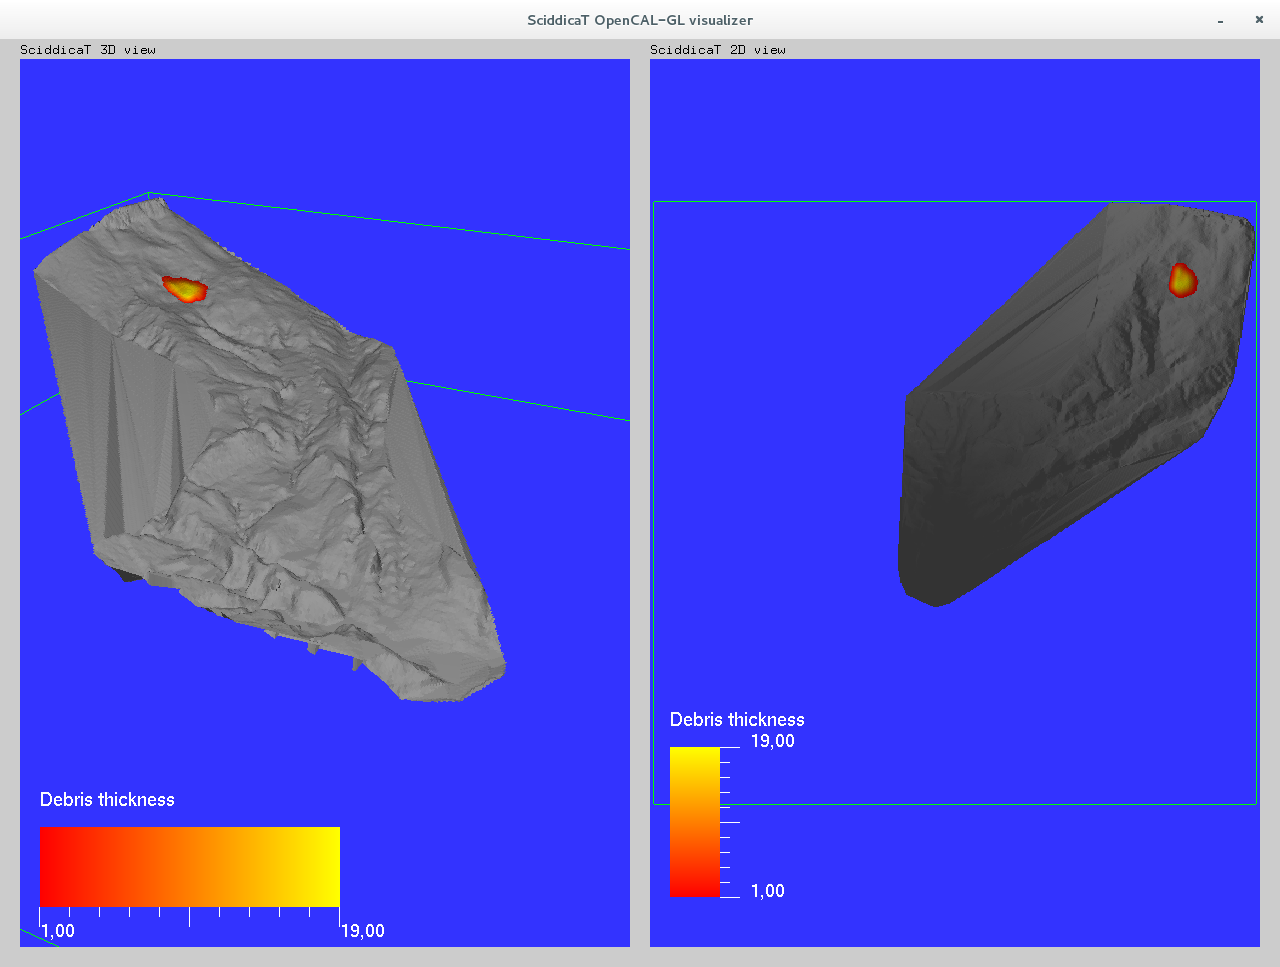
\includegraphics[width=11.4cm]{./images/OpenCAL/calgl_sciddicaT1}
    \caption{Screenshot of the SciddicaT debris flow model with a
      multi-view 2D and 3D visualization system based on OpenCAL-GL.}
    \label{fig:calgl_sciddicaT2}
  \end{center}
\end{figure}


\section{A three-dimensional example}

This section describes the implementation of a simple 3D model, namely
the \emph{mod2} 3D CA, already presented and implemented by means of
the serial version of OpenCAL in Section \ref{sec:mod2}. As for the
previous example about SciddicaT, the \emph{mod2} application comes
together with an OpenCAL-GL-based GUI and 3D rendering system. The
complete source codes for host- and device-side applications are shown
in Listings \ref{lst:calcl_gl_mod2} and
\ref{lst:calcl_gl_mod2_kernel}, respectively .


\lstinputlisting[label=lst:calcl_gl_mod2, caption=An OpenCAL-CL
  implementation of the mod2 3D CA with openCAL-GL graphic
  output.]{../opencal-examples/OpenCAL-CL/calcl_gl_mod2CA3D/source/mod2CA3D.c}

\lstinputlisting[label=lst:calcl_gl_mod2_kernel, caption=The OpenCAL-CL
  kernel implementing the mod2 3D CA elementary
  process.]{../opencal-examples/OpenCAL-CL/calcl_gl_mod2CA3D/kernel/source/mod2CA.cl}


As noted, the host code is quite similar to that of the Game of Life (cf. Section
\ref{sec:calcl_life}), with the difference that here some OpenCAL-GL
code is added for GUI and 3D graphic rendering, as already done for
the $SciddicaT_{naive}$ example (cf. Section
\ref{sec:calcl_sciddicaT}).

The main difference with respect the previous examples is that
\emph{mod2} is a 3D CA model. In fact, the 3D versions of the
previously considered 2D headers are included at lines 3-7 and,
accordingly, the host and device CA, as well as the single model
substate, are declared as 3D objects at lines 18-21. Eventually, note
that also library functions are in their 3D versions. Their meaning is
self-explaining, since they correspond to their 2D counterparts already
seen in previous examples.

Similarly, device-side code is equivalent to that of the Game of
Life. However, since \emph{mod2} is a 3D CA, the kernel in Listing
\ref{lst:calcl_gl_mod2_kernel} also gets the third integer coordinate
for the cell being processed at line 11, by means of the
\verb'calclGlobalSlice()' function. Eventually, as for the host-side
code, even the device-side library functions come in their 3D version.

\verb'OpenCAL-GL/calgl3D.h' and \verb'OpenCAL-GL/calgl3DWindow.h'
headers are included. Moreover, the OpenCAL-GL functions, already seen
in the 2D version in previous Section, are here in their 3D form (see,
e.g., the \verb'calglAdd3Db()' function at line 80). They
are completely equivalent to the 2D versions and therefore will
not be commented. Eventually, note that statements at lines 86-91 are
commented. If comments are removed, you will end with some parts of
the cellular space cut down from the visualization.

Figure \ref{fig:calgl_mod2} shows a screenshot of the \emph{mod2} CA.

\begin{figure}
  \begin{center}
    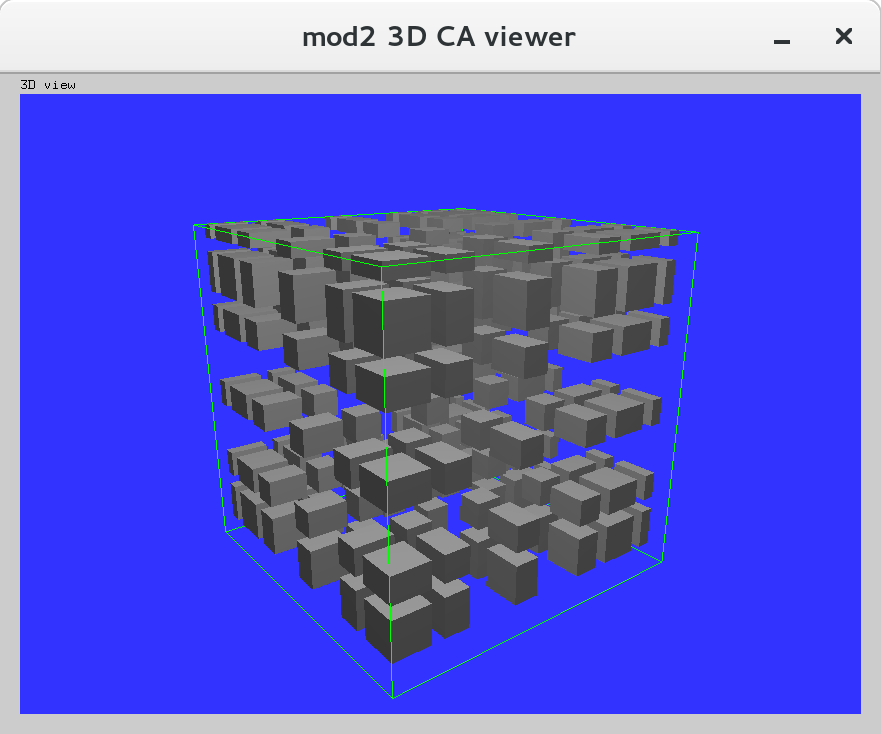
\includegraphics[width=10cm]{./images/OpenCAL/calgl_mod2}
    \caption{Screenshot of the \emph{mod2} 3D CA viewer based on
      OpenCAL-GL.}
    \label{fig:calgl_mod2}
  \end{center}
\end{figure}


\section{Computational performance}
Currently under EVALATE (cit. Beppe Zito).


\section{Reduction operations}
OpenCAL-CL comes with some predefined global reduction operations. In
order to use them, each desired reduction must be firstly registered
to the device-side CA object, by specifying the substate on which the
reduction has to be performed. Registered reductions are performed by
OpenCAL-CL device-side in a transparent way to the user at each
computational step, just after the application of elementary processes
and before steering. Hence, reduction operation results are
retrieved device-side within kernels by means of other predefined
OpenCAL-CL functions. Host- and device-side reduction registration and
retrieving functions are listed in Tables
\ref{tab:calcl-host-reductions} and \ref{tab:calcl-device-reductions},
respectively.


\begin{table}
  \centering
  \footnotesize
  \begin{tabular}{l|l}
    \hline
    Host-side reduction functions & Register a reduction to compute the ... \\
    \hline
    \verb'calclAddReductionMax2Dr()'        & maximum of a substate elements\\
    \verb'calclAddReductionMin2Dr()'        & minimum of a substate elements\\
    \verb'calclAddReductionSum2Dr()'        & sum of a substate elements\\
    \verb'calclAddReductionProd2Dr()'       & product of substate elements\\
    \verb'calclAddReductionLogicalAnd2Dr()' & logical AND of substate elements\\
    \verb'calclAddReductionBinaryAnd2Dr()'  & binary AND of substate elements\\
    \verb'calclAddReductionLogicalOr2Dr()'  & logical OR of substate elements\\
    \verb'calclAddReductionBinaryOr2Dr()'   & binary OR of substate elements\\
    \verb'calclAddReductionLogicalXOr2Dr()' & logical AND of substate elements\\
    \verb'calclAddReductionBinaryXor2Dr()'  & binary AND of substate elements\\
    \hline
  \end{tabular}
  \caption{OpenCAL-CL host-side reduction registration functions for 2D CA and
    substates containing floating point values. In order to obtain the
    corresponding functions for 3D CA, you need to change 2D in 3D
    into the functions' suffix, while to obtain the equivalent
    versions for the other supported basic data types, change the last
    suffix character from r to b or i, for CALbyte- or CALint-based
    substates, respectively.}
  \label{tab:calcl-host-reductions}
\end{table}


\begin{table}
  \centering
  \footnotesize
  \begin{tabular}{l|l}
    \hline
    Device-side reduction functions & Get the value of a reduction operation for the ... \\
    \hline
    \verb'calclGetMax2Dr()'        & maximum of a substate elements\\
    \verb'calclGetMin2Dr()'        & minimum of a substate elements\\
    \verb'calclGetSum2Dr()'        & sum of a substate elements\\
    \verb'calclGetProd2Dr()'       & product of substate elements\\
    \verb'calclGetLogicalAnd2Dr()' & logical AND of substate elements\\
    \verb'calclGetBinaryAnd2Dr()'  & binary AND of substate elements\\
    \verb'calclGetLogicalOr2Dr()'  & logical OR of substate elements\\
    \verb'calclGetBinaryOr2Dr()'   & binary OR of substate elements\\
    \verb'calclGetLogicalXor2Dr'   & logical AND of substate elements\\
    \verb'calclGetBinaryXor2Dr()'  & binary AND of substate elements\\
    \hline
  \end{tabular}
  \caption{OpenCAL-CL device-side reduction retrieving functions for 2D CA and
    substates containing floating point values. In order to obtain the
    corresponding functions for 3D CA, you need to change 2D in 3D
    into the functions' suffix, while to obtain the equivalent
    versions for the other supported basic data types, change the last
    suffix character from r to b or i, for CALbyte- or CALint-based
    substates, respectively.}
  \label{tab:calcl-device-reductions}
\end{table}


Note that, host-side reduction functions return void and accept a
pointer to a device-side CA object and a 0-based numerical handle
corresponding to the device-side substate over which the reduction
must be performed. Instead, device-side reduction retrieving functions
return a CALreal value and only take the 0-based numerical handle
corresponding to the device-side substate over which the reduction has
been performed. Listings \ref{lst:calclAddReductionSum2Dr} and
\ref{lst:calclGetSum2Dr} show the prototypes of the host- and
device-side reductions for evaluating the sum of a substate elements,
respectively. Eventually, Listings
\ref{lst:calcl_reduction_example_host} and
\ref{lst:calcl_reduction_example_device} show a host- and device-side
example codes, respectively, in which a reduction operation is
considered for evaluating the sum of all the elements within a given
substate.

\begin{lstlisting}[float,floatplacement=H, label=lst:calclAddReductionSum2Dr, caption=The calclAddReductionSum2Dr() host-side reduction registration function., numbers=none]
  void calclAddReductionSum[2D|3D][b|i|r](struct CALCLModel2D * device_CA, int devide_side_substate_handle);
\end{lstlisting}

\begin{lstlisting}[float,floatplacement=H, label=lst:calclGetSum2Dr, caption=The calclGetSum2Dr() device-side reduction retriving function., numbers=none]
  CALreal calclGetSum[2D|3D][b|i|r](int device_side_substate_handle);
\end{lstlisting}



\begin{lstlisting}[float, label=lst:calcl_reduction_example_host, caption=An example of global reduction operation in a host-side OpenCAL-CL application.]
  #include <OpenCAL-CL/calcl2D.h>
  #include <OpenCAL-CL/calcl2DReduction.h>
  //...

  // 0-based numerical handle to reger the Q substate device-side
  #define DEVICE_Q 0

  
  int main()
  {
    // ...
    
    // Define a device-side CA
    struct CALCLModel2D * device_CA = calclCADef2D(host_CA, context, program, device);

    // Extract a kernel from program
    CALCLkernel kernel_life_transition_function = calclGetKernelFromProgram(&program, KERNEL_LIFE_TRANSITION_FUNCTION);

    // Register a transition function's elementary process kernel
    calclAddElementaryProcess2D(device_CA, &kernel_life_transition_function);

    // Register reduction operation to be computed after alementary processes and after steering
    calclAddReductionSum2Di(device_CA, DEVICE_Q);

    //...
  }
\end{lstlisting}


\begin{lstlisting}[float, label=lst:calcl_reduction_example_device, caption=An example of global reduction operation in a device-side OpenCAL-CL application.]
  #include <OpenCAL-CL/calcl2D.h>
  #include <OpenCAL-CL/calcl2DReduction.h>
  

  // 0-based numerical handle to reger the Q substate device-side
  #define DEVICE_Q 0

  __kernel void lifeTransitionFunction(__CALCL_MODEL_2D)
  {
    calclThreadCheck2D();
    
    int i = calclGlobalRow();
    int j = calclGlobalColumn();

    // retrieve and print the result of the sum reduction
    // operation registered host-side
    int sum = calclGetSum2Di(DEVICE_Q);
    if(i==0 && j==0) 	
      printf("sum = %f \n", sum);

    //...
  } 
\end{lstlisting}
